\chapter{Embedding}
\label{chap:embed}
In this chapter we will cover the various processes by which we go from general Hamiltonians like the ones from Chapter \ref{chap:aqc} to Hamiltonians which will fit on the \machine as described in Chapter \ref{chap:machine}.

\section{Creating Problem Hamiltonians}
Embedding is the name we give to the general process of translating a computational problem into something which is ready for an adiabatic quantum computer to evaluate.  As mentioned in Section \ref{sec:prob_ham}, the first step is to generate a problem Hamiltonian.  We employ two methods for finding suitable problem Hamiltonians.  The first, using linear programming, is suitable for small Hamiltonians (generally only a few variables in size).  The second is to use the software \texttt{QCC} which takes advantage of the gluing theorem to stitch together a problem Hamiltonian out of smaller sub-Hamiltonians.
The second step in the embedding process is to translate our problem Hamiltonians, which generally may have arbitrary topologies, coupling values, number of variables etc. into Hamiltonians which the \machine is capable of physically implementing.

These are not the only methods of generating problem Hamiltonians.  The programmatic style described above seems natural for solving actual computational problems, but e.g. if one wanted to go a more academic computer science route one could reduce one's problems to known NP-Complete problems and evaluate those.  Lucas \cite{lucas} handily provides a compilation of ising formulations of a variety of different NP-Complete suitable for such an approach.

\section{Linear Programming}
\label{sec:lin_prog}
The requirements we have for a problem Hamiltonian can be described using a system of constraints, and solved using the techniques of linear programming (LP).
Briefly, LP is a method to optimize some objective function subject to linear equality and linear inequality constraints.  There are three standard parts that describe a linear programming problem:

\begin{itemize}
	\item A linear function to be maximized or minimized
		\subitem $f(x_0,x_1) = c_0x_0 + c_1x_1$
	\item Constraint Matrix $A$:
		\subitem $A\vec{x} \le \vec{b} $
	\item Non-negative variables
		\subitem $x_i \ge 0$ $\forall i$
\end{itemize}


(thus the name \emph{linear} programming).  There are many software packages that implement LP solving, both Free Software and proprietary.  This makes it an easily accessible technique.

To use linear programming to create a problem Hamiltonian with N spins we first assign a variable $x_i$ for each field and each coupling that could be in the end result; this is $N(N-1)/2 + N$ or $N(N + 1)/2$ ($N$ choose $2 + N$ variables).  Then we add a constraint for each possible assignment of the spins, making $2^N$ constraints.  In these constraints we have every sign combination of the variables that correspond to fields, e.g.

\begin{align}
	 c_0 &  = x_0 + x_1 + x_2 \nonumber \\ 
	 c_1 & = x_0 + x_1 - x_2 \nonumber \\ 
	 c_2 & = x_0 - x_1 + x_2 \nonumber \\
	 c_3 & = x_0 - x_2 - x_2 \\
		 & \mathrm{etc.} \nonumber
\end{align}

In each constraint we also add the variables representing couplings; the sign of each coupling variable should be the product of the two variables that represent the two spins the coupling connects.  Now for each state which we want to be part of the ground state we set the value of the constraint equal to $k$; for each state that is \emph{not} part of the ground state, we enforce that the corresponding constraint is strictly greater than $k$.  

For example, if we know the truth table for a \texttt{NAND} gate and want to find a set of fields and couplings that create a matching Hamiltonian, the constraints would be

\begin{align}
	c_0 &= -x_0 - x_1 - x_2 + x_3 + x_4 + x_5 + k &\ge 1 \nonumber\\
	c_1 &= -x_0 - x_1 + x_2 + x_3 - x_4 - x_5 + k &= 0 \nonumber\\
	c_2 &= -x_0 + x_1 - x_2 - x_3 + x_4 - x_5 + k &\ge 1 \nonumber\\
	c_3 &= -x_0 + x_1 + x_2 - x_3 - x_4 + x_5 + k &= 0 \nonumber\\
	c_4 &= x_0 - x_1 - x_2 - x_3 - x_4 + x_5 + k &\ge 1 \nonumber\\
	c_5 &= x_0 - x_1 + x_2 - x_3 + x_4 - x_5 + k &= 0 \nonumber\\
	c_6 &= x_0 + x_1 - x_2 + x_3 - x_4 - x_5 + k &= 0 \nonumber\\
	c_7 &= x_0 + x_1 + x_2 + x_3 + x_4 + x_5 + k &\ge 1 
\end{align}

For all three spin gates the constraints would be identical except for which states are $k = 0$ and which are $k \ge 1$.  This particular set of constraints will produce a \texttt{NAND} gate; each of the variables $x_0, x_1, x_2$ in the constraint equal to zero matches the truth table (see Table \ref{tab:couplings}) for \texttt{AND} with input variables $x_0, x_1$ and output variable $x_2$.

The combined effect of all of these constraints is that when we solve the system for the set of variables $x_i$ which minimize the objective function, states which encode the desired logic will have an energy of $-k$ and states which do not encode the desired logic will have an energy greater than $-k$.
This is a slightly unusual use for LP; normally finding the set of $x_i$'s that optimize the objective function is the goal, but for us finding the $x_i$'s which satisfy the constraints if the central objective.
Minimizing the sum of the coupling values simply helps to keep the number of different coupling values small and the spread between them down.  This will be important because physical adiabatic quantum computers can only implement a finite number of different coupling values in finite ranges. 

Unfortunately while this method allows us to find a set of couplings to encode the logic of any circuit, we require a constraint for each possible state of each of the variables.  For a binary circuit with $n$ variables, there are $2^n$ states.
The above process for creating problem Hamiltonians is thus clearly exponentially hard, and becomes extremely computationally inefficient for larger circuit sizes.
That said, this method retains utility for finding small sub-Hamiltonians to use as building blocks for larger problem Hamiltonians using \texttt{QCC} as described in the next section.

\section{\texttt{QCC}}
\texttt{QCC} is a collection of programs and libraries designed to produce problem Hamiltonians.  The core of \texttt{QCC} are two pieces: the \texttt{QSM} language and interpreter, and the embedding algorithm.  The \texttt{QSM} language is a programming language designed to simplify the connecting of sub-Hamiltonians.  It is both human writable and serves as a compilation target for more complicated or high level languages.  One can write a \texttt{QSM} file describing a circuit composed of multiple sub-Hamiltonians, and the \texttt{QSM} interpreter will construct the appropriate problem Hamiltonian, including any auxiliary spins that the sub-Hamiltonians need.  Once the problem Hamiltonian has been generated, a Hamiltonian with equivalent ground states that is isomorphic to a sub-graph of a particular hardware implementation must be created in order for the problem Hamiltonian to be solved; this is the job of the embedding algorithm.

\section{\texttt{QSM} Language}
The \texttt{QSM} language is a simple language designed to be readable and writable by both humans and machines.  A \texttt{QSM} file consists of one or more \texttt{QSM} statements; each \texttt{QSM} statement is enclosed by parentheses and consists of a whitespace separated list of the statement components.  If a component has multiple sub-parts then they are also enclosed in parentheses.  There are two kinds of \texttt{QSM} statements, gate statements and clamp statements.

A typical \texttt{QSM} gate statement consists of three components: first the name of the gate or sub-Hamiltonian to be included, then a parenthesis-enclosed list of the input spins for the gate, and third a parenthesis-enclosed list of the output spins for the gate.  An example \texttt{QSM} gate statement is: 
\begin{center}
	\texttt{(and (a b) (c))}
\end{center}
This \texttt{QSM} statement encodes the logic $A \wedge B = C$.  A variable name may be prefixed by a $\sim$, in which case the logic of that variable is negated.  The other type of \texttt{QSM} statement besides a gate statement is the clamp statement; this statement consists of two components.  First the keyword \texttt{clamp}, followed by a list of variables and the values that they are to be clamped to.  A clamp statement looks like
\begin{center}
	\texttt{(clamp ((a +1) (b -1)))}
\end{center}
The above clamp statement sets the value of the variables \texttt{a} and \texttt{b} to +1 and -1, respectively.

A complete \texttt{QSM} file might then look like

\begin{center}
	\texttt{(and (A $\sim$B) (C))}\\
	\texttt{(or (X Y) (B))}\\
	\texttt{(clamp ((C +1)))}
\end{center}
which would compile to a Hamiltonian which encodes the logic $A \wedge \neg B = C, X \vee Y = B, C = \text{TRUE}$ and the resulting ground states will be those states for which the logic is satisfied.

Figure \ref{fig:eg_embed} shows the shape of the resulting graph.  The node for $C$ is greyed out to represent the fact that it is clamped.  Each of the input sub-Hamiltonians (\texttt{and} and \texttt{or}) connect each of the spins they're given, and the resulting shape has node $B$ connected to every other node, $X$ and $Y$ connected to each other, and $A$ only connected to $B$.  This Hamiltonian graph does not have the same shape as the \machine graph, and so will have to be embedded in the following section.

\begin{figure}
	\begin{center}
		\scalebox{0.5}{
			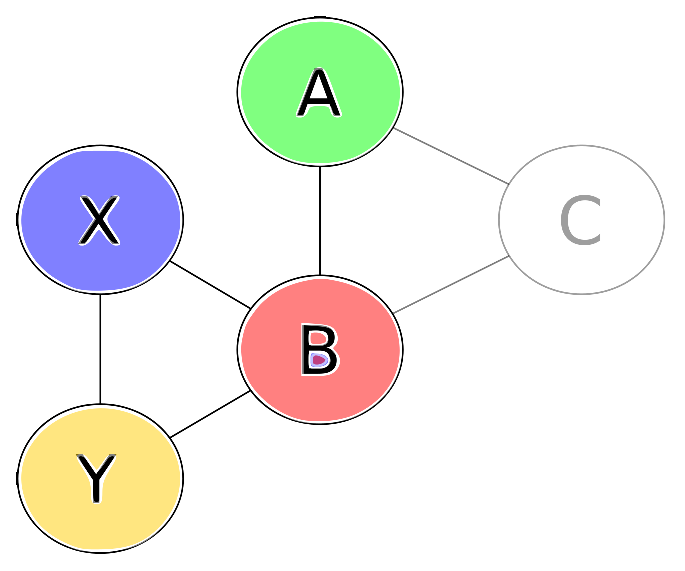
\includegraphics{img/eg_embed.eps}
		}
	\end{center}
	\caption[Embedding example]{The shape of an example Hamiltonian as would be created by \texttt{QCC}.  This graph will not fit on the \machine, so in the next section we will demonstrate the embedding algorithm on it.}
	\label{fig:eg_embed}
\end{figure}

\section{Embedding algorithm}
\label{sec:embed_algo}
Once we have our problem Hamiltonians we need to convert them into Hamiltonians which have the same shape as the graph that the \machine machine has.  This is done by adding \emph{clone spins} into the graph: each clone spin has the same value in the ground state as one of the logical spins in the input graph.  
This allows us to decrease the connectivity of the problem Hamiltonian until it is sparse enough to be the same shape as the physical machine.  The following algorithm is essentially equivalent to one presented in \cite{choi1}.
We expect that translating complete graphs onto graphs with constant connectivity to require roughly a quadratic size penalty in the number of clone spins (as the number of connections in a complete graph is $\sim n^2$).
Ideally, to ensure that each clone spin's ground state is the same as it's parent we would have $J_{ij} << J_{clone} \forall i,j$.  Because of physical limits of the machine (especially the resolution mentioned in Section \ref{sec:resolution}) large values of $J_{clone}$ may not maximize fidelity: for a machine with finite resolution, having a large $J_{clone}$ may compress other coupling values together such that the ground state starts to overlap with higher energy state.  On the other hand a too small value of $J_{clone}$ may result in ground states in which the clones are not aligned, which will almost certainly also produce incorrect ground states. Thus we have to find an empirical value of $J_{clone}$ that maximizes the fidelity while preserving the ground states.

\begin{figure}
	\begin{tabular}{l l l}
		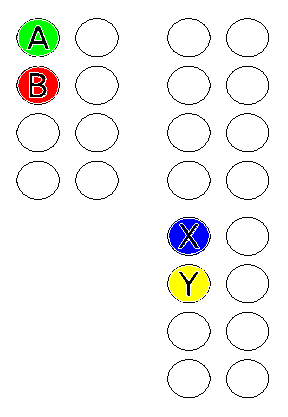
\includegraphics{img/eg_embed_full.eps} & \hspace{1 in} &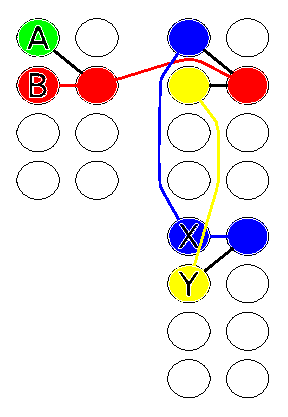
\includegraphics{img/eg_embed_full2.eps} \\
	\end{tabular}
	\caption[Embedding Algorithm]{This figure shows two steps in the embedding process.  On the left is the first step, assigning elements of the input graph (Figure \ref{fig:eg_embed}) along the diagonal of the \machine graph.  On the right is the connection step; nodes with the same colour share logical values.  Coloured lines represent the \emph{clone couplings}, while black lines represent the computational couplings.}
	\label{fig:embedding}
\end{figure}

Figure \ref{fig:embedding} shows a demonstration of the embedding algorithm.  The main idea is to assign nodes from the Hamiltonian you are trying to embed along the diagonal of the \machine graph.  Then link up connected nodes by cloning right and up from the nodes that need to be connected.

The embedding algorithm is as follows:

\emph{\textbf{Definitions:}}

Designate the input Hamiltonian graph $V$ and the output graph $G$.  Label the spins in $V$ and $G$ as $V_i$ and $G_i$ respectively.
We define the \emph{clone map} $C_i$ as the set of spins $[i,j \ldots]$ which have the same logical value as their parent spin: so for example the clone map of spin 5, $C_5$, might be $[2,3,13]$ which would mean that spins 2, 3, 5 and 13 all share the same logical value.  
We define a mapping $M$ between logical spins in graph $V$ and computation spins in graph $G$.  For example, spin $V_{12}$ representing the 12th variable in a problem might be mapped to $G_{187}$, the 187th machine spin.

We also define a \emph{clone coupling} value which is as large as possible and ferromagnetic; this attempts to ensure that all the members of a clone map are aligned in the ground state.  In the final $G$, each member of a clone map should have a clone coupling connecting it to at least one other member of the clone map.

\emph{\textbf{Procedure:}}
\begin{enumerate}
	\item Populate $M$ by mapping each $V_i$ to one of the spins $G_j$ on the left side of a unit cell that lies along the diagonal of $G$
	\item For each field term in $V$, add a field to $G$ on the corresponding spin
	\item For each $J_{ij}$ in $V$, conduct the following operation:
		\begin{itemize}
			\item Scan through both of $C_i$ and $C_j$ to find the pair which are nearest to each other in $G$; call these $x$ and $y$
			\item Get a list of each spin that lies along the path between $x$ and $y$
			\item Assign half of these spins to $C_i$ and half to $C_j$; add the appropriate clone coupling into $G$ for each spin in the path to ensure that the clone map is properly connected
			\item Finally, at the interface between the two new clone map members, add a coupling into $G$ with the same value as $J_{ij}$
		\end{itemize}
\end{enumerate}

Each term in $V$, both fields and couplings, should now have a corresponding term in $G$.  $G$ should also contain many coupling terms that group the necessary clone maps.  

This algorithm is tailored to AQC machines whose qubits are arranged in a square shape (specifically the shape of the \machine), however, the principle should be generalizable: as mentioned above any reasonably compact graph with constant connectivity should be able to embed a complete graph with an $n^2$ overhead by allocating the input graph spins along the diagonal.
